\documentclass[11pt, a4paper, oneside]{report}

% --- Core Packages ---
\usepackage[utf8]{inputenc}
\usepackage[T1]{fontenc}
\usepackage{geometry}
\geometry{margin=1in}
\usepackage{helvet} 
\usepackage{hyperref}
\usepackage{graphicx}
\usepackage{listings}
\usepackage{xcolor}
\usepackage{titlesec}
\usepackage{fancyhdr}
\usepackage{amsmath}

% --- Path for Screenshots ---
\graphicspath{{./screenshots/}}

% --- Styling Colors ---
\definecolor{brandblue}{rgb}{0.12, 0.29, 0.49}
\definecolor{codebg}{rgb}{0.96, 0.96, 0.98}
\definecolor{commentgreen}{rgb}{0.0, 0.5, 0.0}

% --- Hyperref Setup ---
\hypersetup{
    colorlinks=true,
    linkcolor=brandblue,
    urlcolor=cyan,
    pdftitle={WYI Project System Manual},
}

% --- Code Listing Config ---
\lstset{
    backgroundcolor=\color{codebg},   
    commentstyle=\color{commentgreen},
    keywordstyle=\color{blue}\bfseries,
    basicstyle=\ttfamily\small,
    breaklines=true,        
    frame=single,
    captionpos=b,                    
    tabsize=2
}

\begin{document}

\title{
    \Huge \textbf{WYI System Manual} \\
    \vspace{1cm}
    \Large Intelligent Bill Management and Review Platform \\
    \large F\# Backend + Vue.js Frontend + Gemini AI
}
\author{SIDUO CHEN (Lao Chen)}
\date{April 2026}

\maketitle

\chapter{Project Overview}
\section{Objective}
The WYI platform automates financial document recognition and validation using the Google Gemini 1.5 Flash model. It aims to eliminate manual data entry in bill negotiation workflows by extracting structured information from raw images and PDFs.

\section{Resource Links}
\begin{itemize}
    \item \textbf{Production URL:} \url{https://whatsyourideal.com/}
    \item \textbf{Demo URL:} \url{https://5.78.201.21/}
    \item \textbf{Main Repository:} \url{https://github.com/R77R77R/WYI/}
    \item \textbf{JCS Code Generator:} \url{https://github.com/lchenmay/JCS/}
    \item \textbf{Common Library:} \url{https://github.com/lchenmay/Common/}
\end{itemize}

\chapter{Authentication and User Onboarding}
The system utilizes Clerk.js for identity management. This ensures secure, industry-standard authentication while allowing users to leverage existing social accounts like Google.

\begin{figure}[h]
    \centering
    
\includegraphics[width=0.7\textwidth]{screenshots/signin-1.png}
    \caption{Initial Sign-in Interface supporting Google and other OAuth providers.}
\end{figure}

\begin{figure}[h]
    \centering
    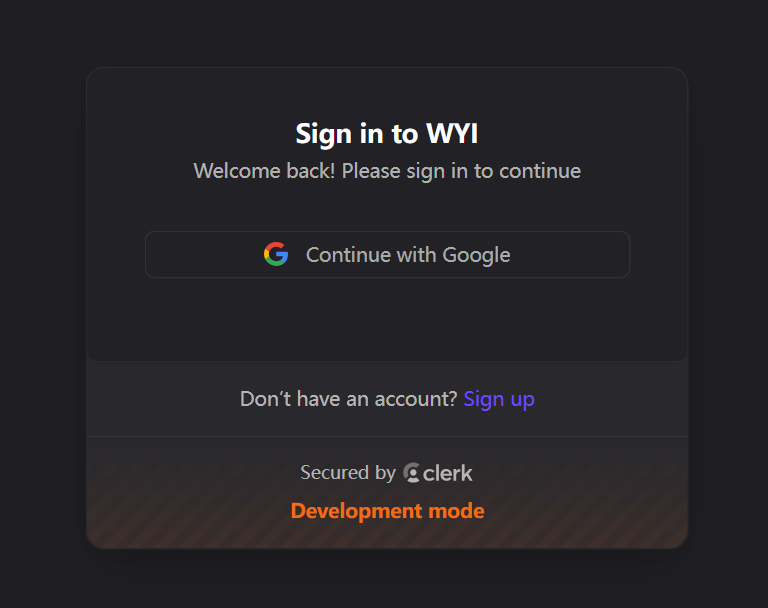
\includegraphics[width=0.7\textwidth]{screenshots/signin-2.png}
    \caption{Official Google Sign-in Page integration.}
\end{figure}

\begin{figure}[h]
    \centering
    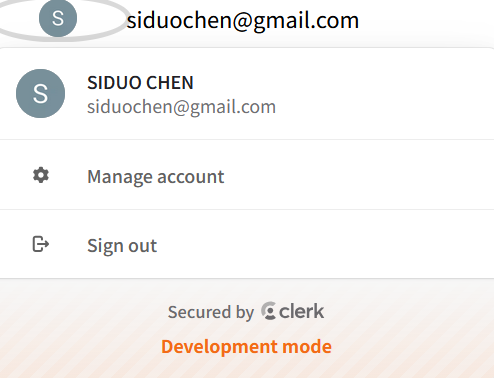
\includegraphics[width=0.7\textwidth]{screenshots/signin-3.png}
    \caption{Authenticated User Session Dashboard showing registered user status.}
\end{figure}

\chapter{System Features}

\section{AI-Driven Bill Review}
The backend orchestrates file processing via the \texttt{reviewBillFiles} module. It extracts fields such as Amount (\texttt{Amt}), Bill Date, and Account Number using the multimodal capabilities of Gemini AI.

\begin{figure}[h]
    \centering
    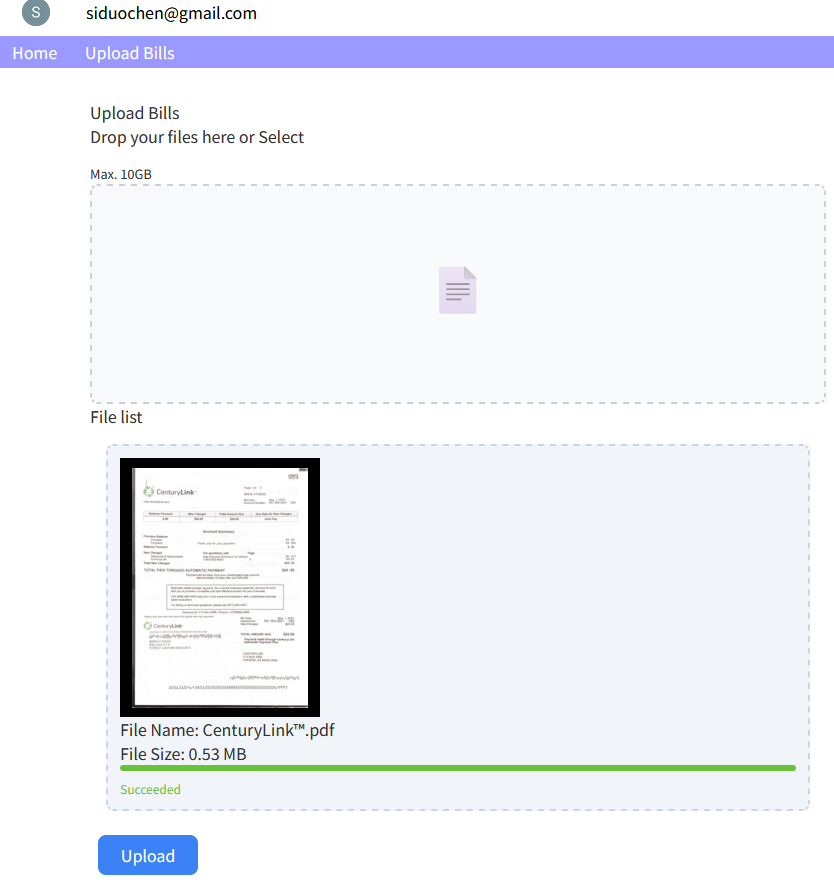
\includegraphics[width=0.8\textwidth]{screenshots/upload-files.png}
    \caption{File Upload Interface: Users can upload bill images or PDFs for analysis.}
\end{figure}

\begin{figure}[h]
    \centering
    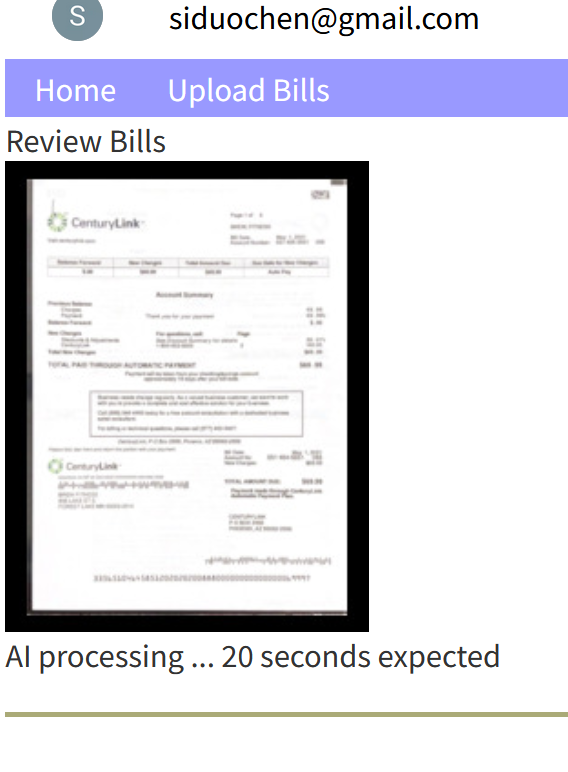
\includegraphics[width=0.8\textwidth]{screenshots/ai-review-1.png}
    \caption{Gemini 1.5 Flash performing multimodal extraction on uploaded bills.}
\end{figure}

\begin{figure}[h]
    \centering
    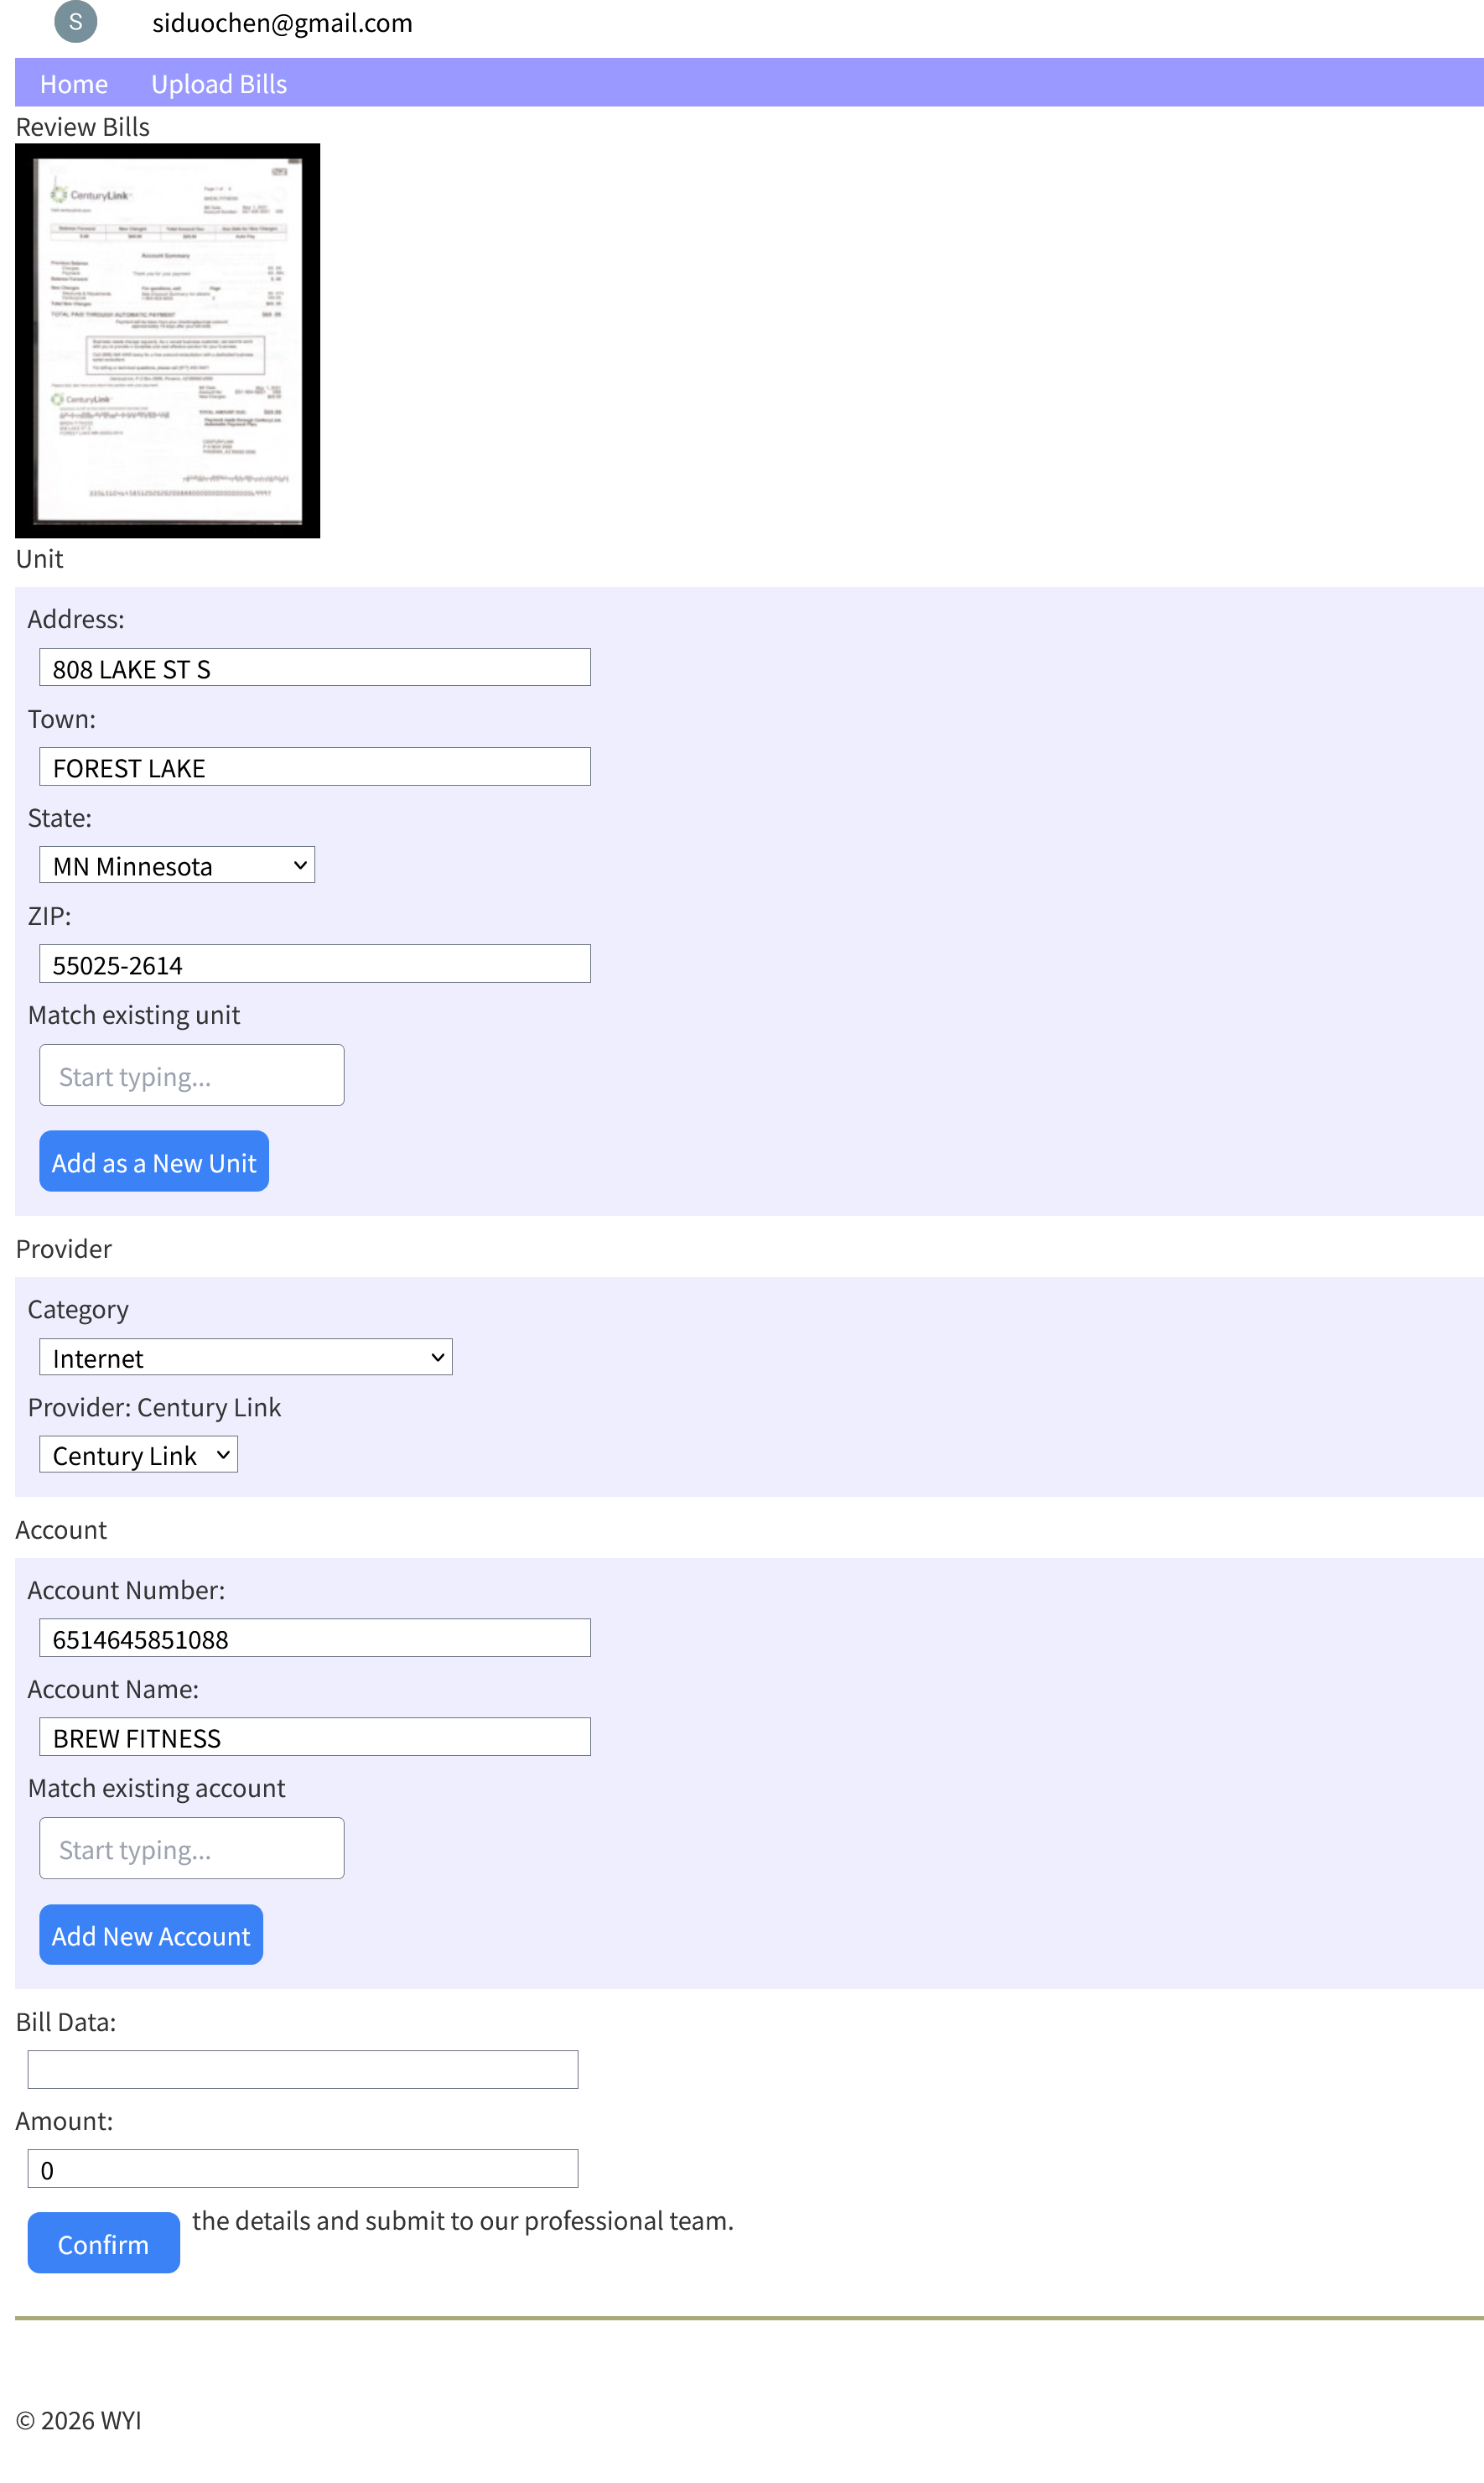
\includegraphics[width=0.8\textwidth]{screenshots/ai-review-2.png}
    \caption{Manual verification interface in Vue.js for AI-extracted data.}
\end{figure}

\section{Data Management}
The system allows users to maintain property units (home, restaurant, office) and service providers, which helps link incoming bills to existing historical data.

\begin{figure}[h]
    \centering
    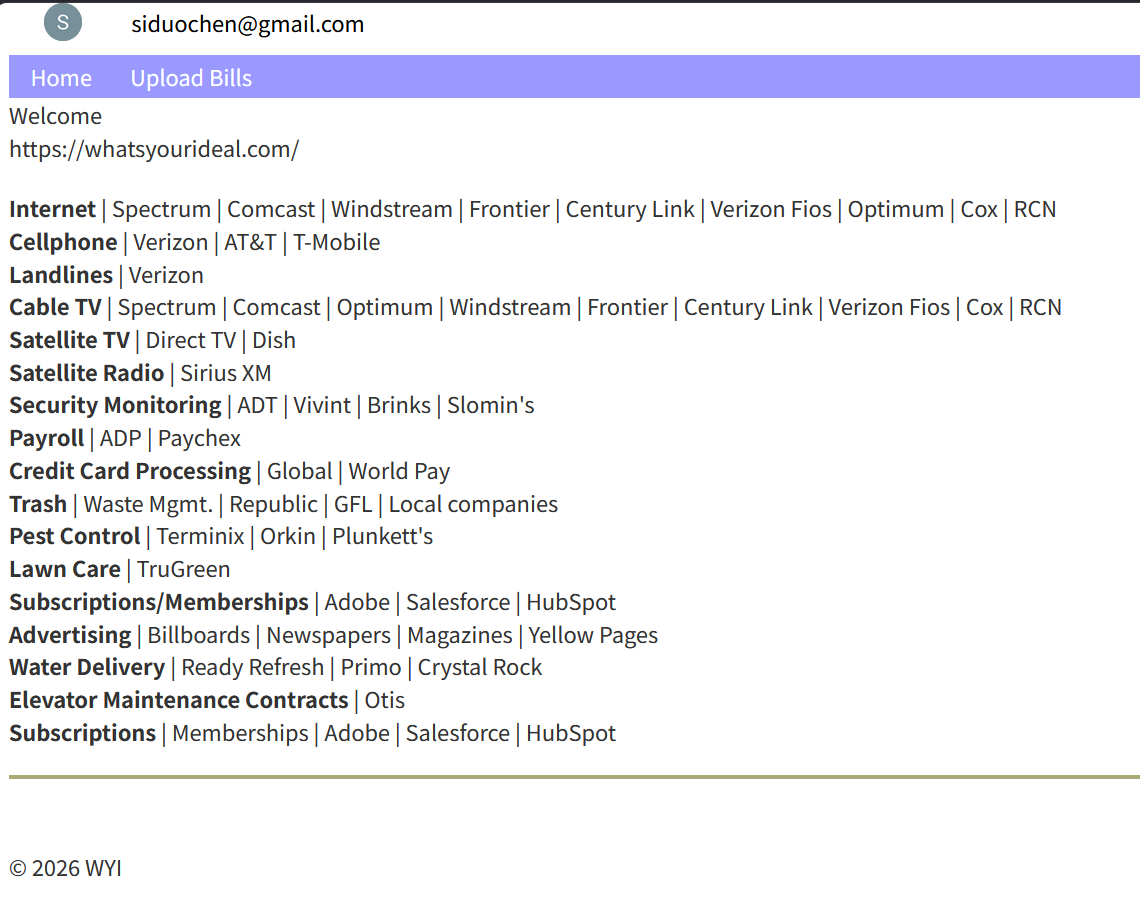
\includegraphics[width=0.7\textwidth]{screenshots/cat-provider.png}
    \caption{Maintenance of Categories and Providers within the database.}
\end{figure}

\begin{figure}[h]
    \centering
    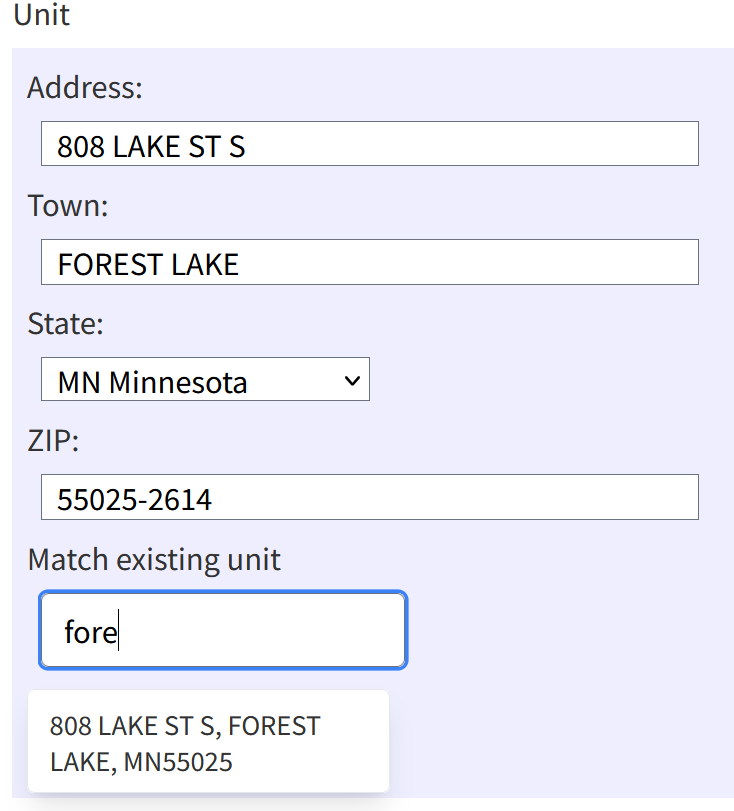
\includegraphics[width=0.7\textwidth]{screenshots/manage-my-unit.png}
    \caption{Property Unit Management Interface (Residential/Commercial).}
\end{figure}

\chapter{Technical Implementation}
\section{Backend Logic (F\#)}
The system uses F\# to handle the coordination between the user context and the AI engine. The \texttt{reviewBillFiles} function manages file paths and invokes the Gemini service.

\begin{lstlisting}[language=ml, caption=F\# Gemini Integration Logic]
// Asynchronous multimodal extraction logic from ApiEu.fs
let reviewBillFiles eux (x:X) =
    // Orchestrates GeminiMultimodal task with a 300s timeout
    let! (ex, msg) = GeminiMultimodal runtime.output apiKey model prompt pathes
\end{lstlisting}

\chapter{Troubleshooting}
\section{AI Usage and Prepayment}
The system operates under a Paid Tier 1 model to ensure reliability.
\begin{itemize}
    \item \textbf{Error 429:} This status occurs when prepayment credits are depleted. All API requests are rejected until funds are added via Google AI Studio.
    \item \textbf{Quota Management:} The system is designed for a capacity of 1,000 RPM and 1M TPM for Gemini 1.5 Flash.
\end{itemize}

\section{Timeout Handling}
The system is configured with a 300-second timeout to accommodate high-resolution multi-file uploads.

\end{document}